\subsection{Feature Selection Experiments}
\label{subsec:pmc-results-feature-selection-experiments}

This section evaluates which input features contribute most to predicting peak memory usage.
The goal is to determine what is the minimum set of features to train a model capable of predicting memory usage, and whether additional shape-derived features improve performance.

Experiments use the best model per operator identified earlier: Gradient Boosting (Envelope), Decision Tree (\ac{GST3D}), and Linear Regression (Gaussian Filter).

\subsubsection{Volume-Centric Hypothesis}
\label{subsec:feature-selection-volume-centric-hypothesis}

Figure~\ref{fig:memory_vs_volume_regression_subplots} shows that memory usage aligns closely with volume across all operators.
This supports the hypothesis that volume alone may be sufficient for reliable prediction.

\begin{figure*}[htbp]
    \centering
    \begin{subfigure}[t]{0.32\textwidth}
        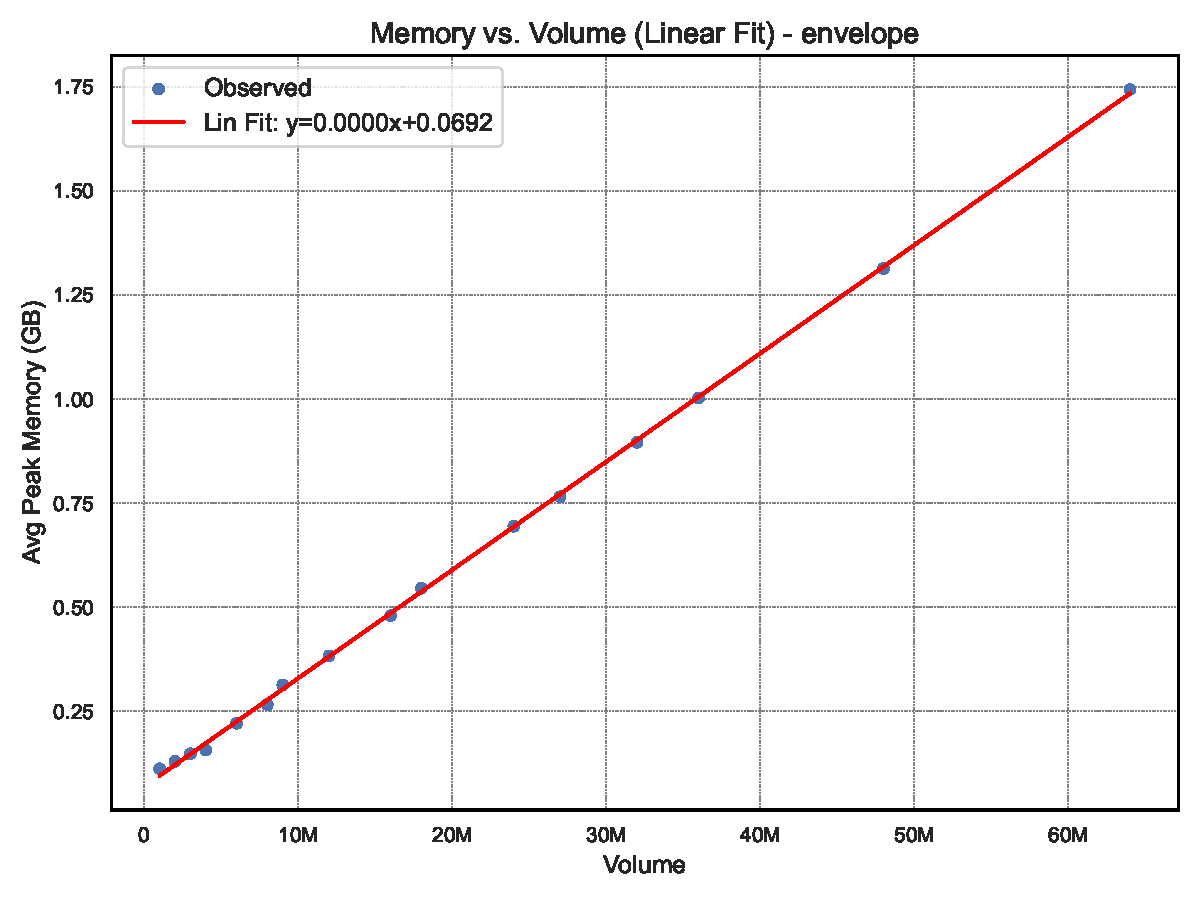
\includegraphics[width=\textwidth]{assets/images/05/memory_vs_volume_regression_envelope}
        \caption{Envelope}
    \end{subfigure}
    \hfill
    \begin{subfigure}[t]{0.32\textwidth}
        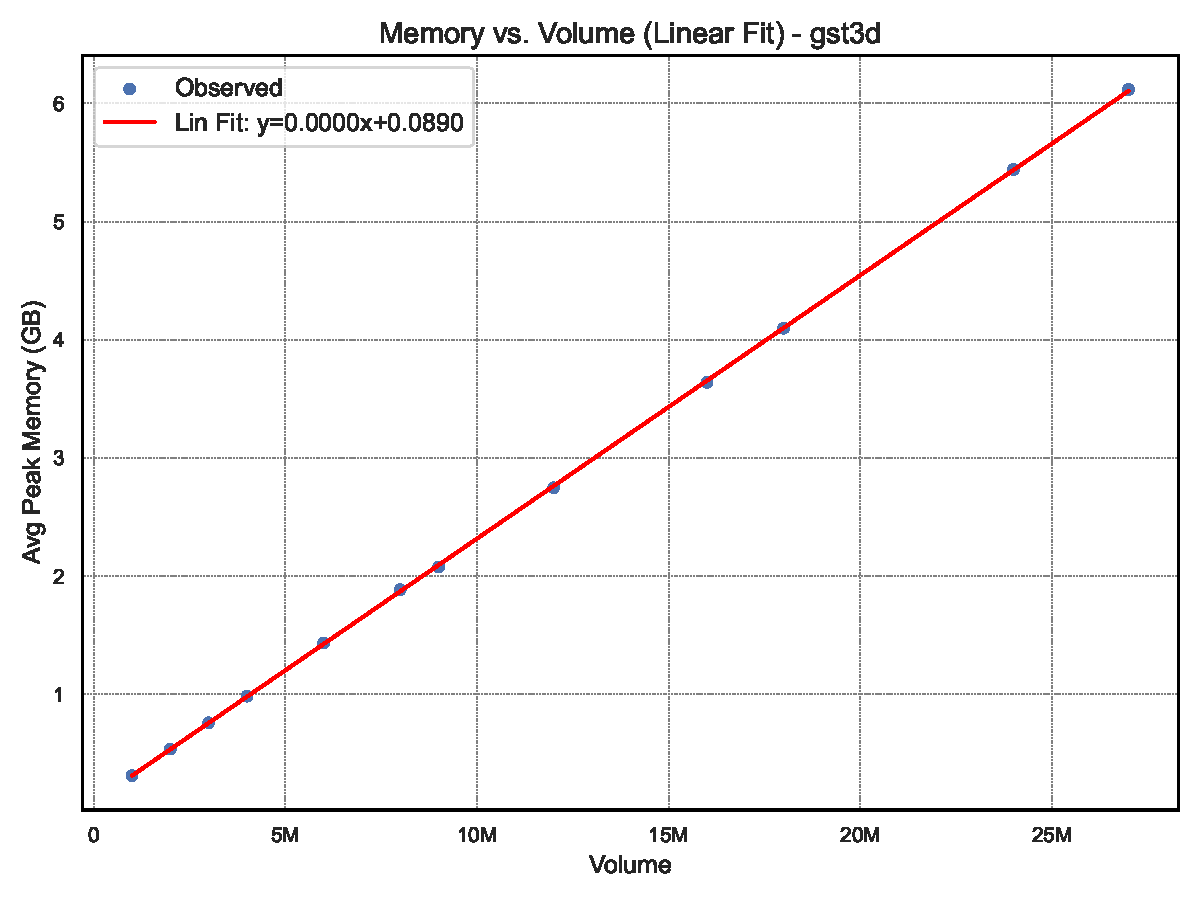
\includegraphics[width=\textwidth]{assets/images/05/memory_vs_volume_regression_gst3d}
        \caption{\ac{GST3D}}
    \end{subfigure}
    \hfill
    \begin{subfigure}[t]{0.32\textwidth}
        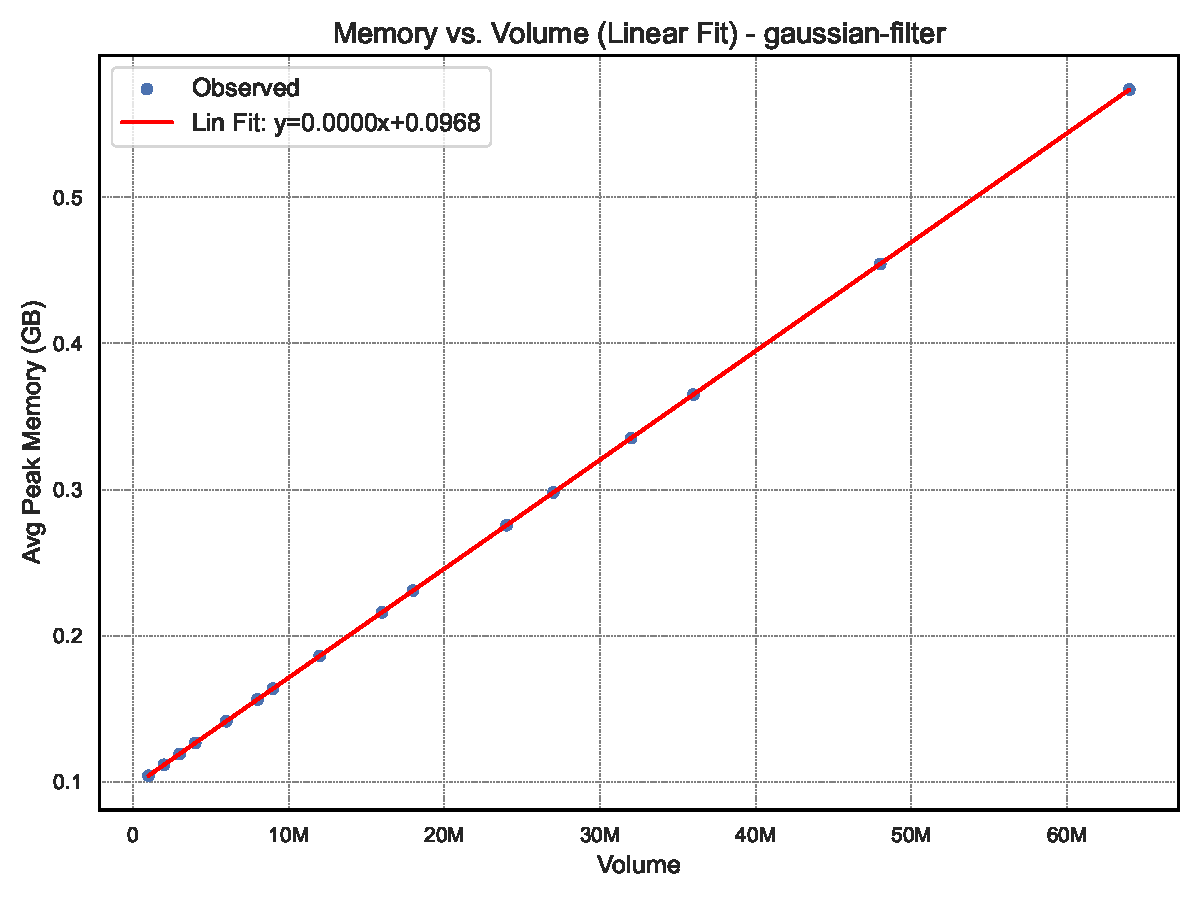
\includegraphics[width=\textwidth]{assets/images/05/memory_vs_volume_regression_gaussian-filter}
        \caption{Gaussian Filter}
    \end{subfigure}
    \caption{Memory usage vs. volume with regression fits. Each operator displays strong linearity.}
    \label{fig:memory_vs_volume_regression_subplots}
\end{figure*}

\subsubsection{Feature Removal Process and Metrics}
\label{subsec:feature-removal-methods-and-metrics}

The feature selection procedure applies a stepwise elimination strategy:

\begin{enumerate}
    \item Rank features using SelectKBest based on their individual predictive power.
    \item Iteratively remove features starting with the least relevant.
    \item Track changes in \ac{RMSE}, $R^2$, accuracy, and score.
    \item Repeat until only feature remains.
\end{enumerate}

Table~\ref{tab:feature_selection_minimal_impact} summarizes example results.
Performance remains stable with just three features, as long as volume is retained.

\begin{table}[htbp]
    \centering
    \begin{tabular}{lccc}
        \hline
        \textbf{Operator} & \textbf{Model}    & \textbf{\#Features} & \textbf{\ac{RMSE} / $R^2$}     \\
        \hline
        Envelope          & Gradient Boosting & 25                  & 0.0167 / 0.9961                \\
        Envelope          & Gradient Boosting & 1                   & 0.0150 / 0.9969                \\
        \ac{GST3D}        & Decision Tree     & 25                  & 0.0023 / 0.999997              \\
        \ac{GST3D}        & Decision Tree     & 1                   & 0.0039 / 0.999992              \\
        Gaussian Filter   & Linear Regression & 25                  & $2.4\times10^{-5}$ / 0.9999999 \\
        Gaussian Filter   & Linear Regression & 1                   & $2.2\times10^{-5}$ / 0.9999999 \\
        \hline
    \end{tabular}
    \caption{Effect of reducing feature count on RMSE and $R^2$. Results remain stable with only a single feature.}
    \label{tab:feature_selection_minimal_impact}
\end{table}

\subsubsection{Impact on RMSE, R\texorpdfstring{$^2$}{2}, and Residuals}
\label{subsec:impact-on-rmse-r2-and-residuals}

Figure~\ref{fig:feature_selection_overview_part1} shows the average RMSE and $R^2$ as features are removed.
Performance never drops significantly, even when reducing to a single feature.

\begin{figure*}[htbp]
    \centering
    \begin{subfigure}[t]{0.49\textwidth}
        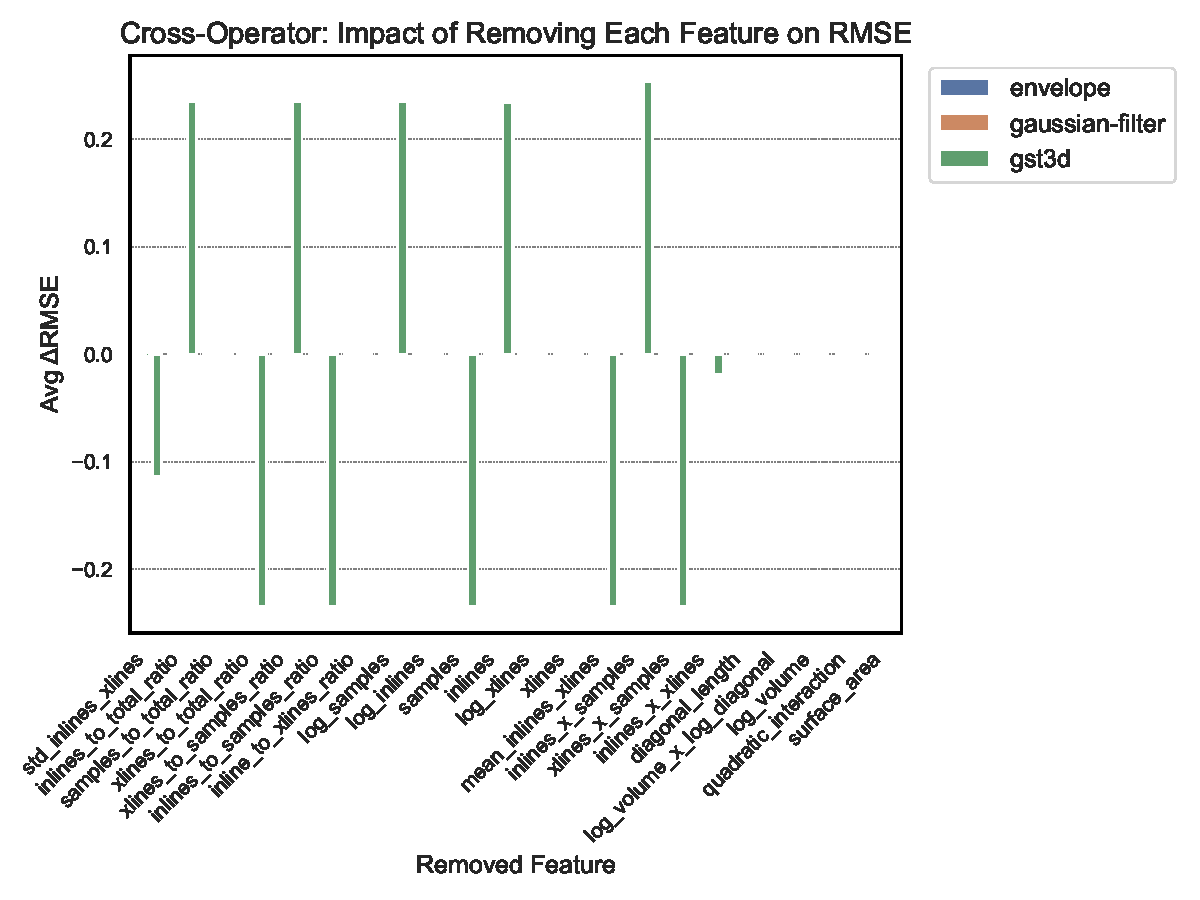
\includegraphics[width=\textwidth]{assets/images/05/feature_impact}
        \caption{Average RMSE change}
    \end{subfigure}
    \hfill
    \begin{subfigure}[t]{0.49\textwidth}
        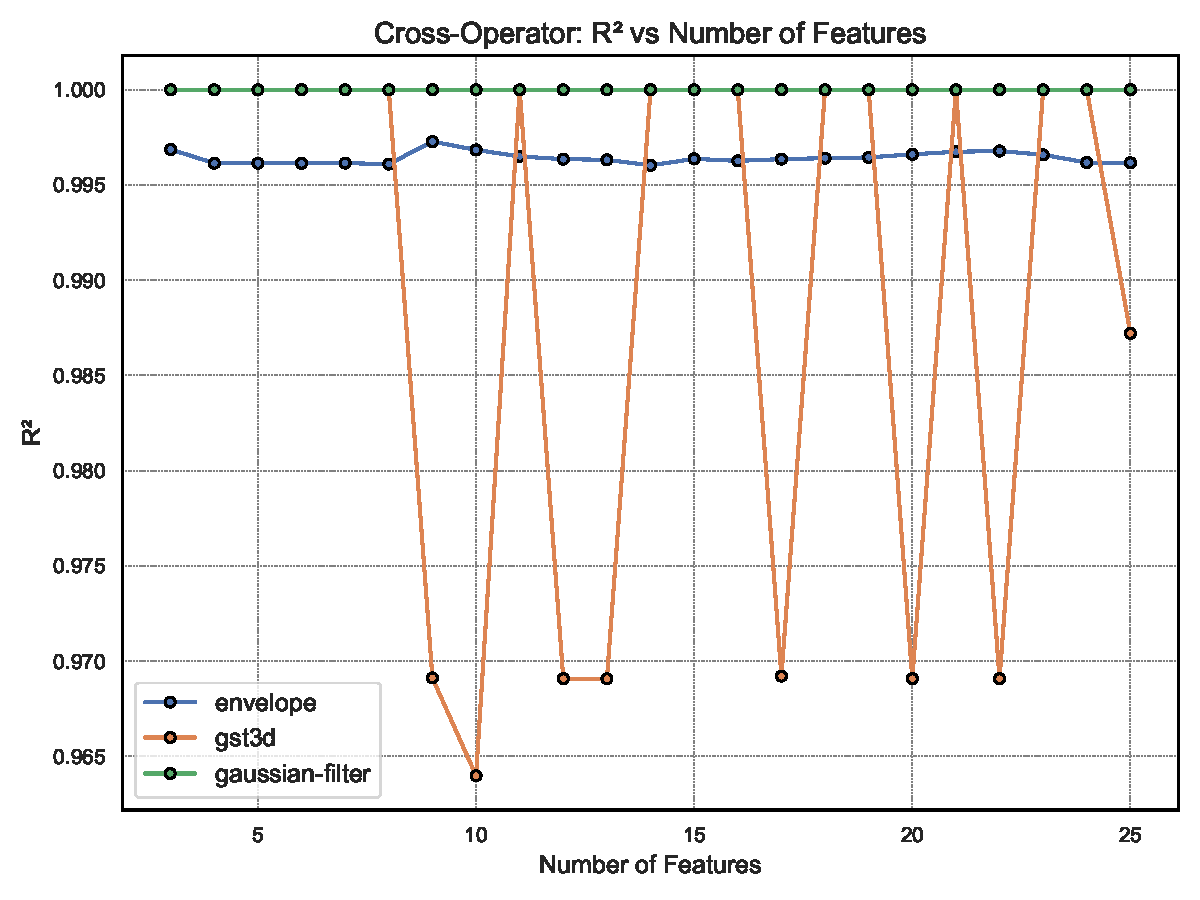
\includegraphics[width=\textwidth]{assets/images/05/cross_feature_selection_r2}
        \caption{Change in $R^2$}
    \end{subfigure}
    \caption{Effect of removing features. Volume is the most critical predictor.}
    \label{fig:feature_selection_overview_part1}
\end{figure*}

Residual metrics and scores remain stable throughout feature reduction.

\begin{figure*}[htbp]
    \centering
    \begin{subfigure}[t]{0.49\textwidth}
        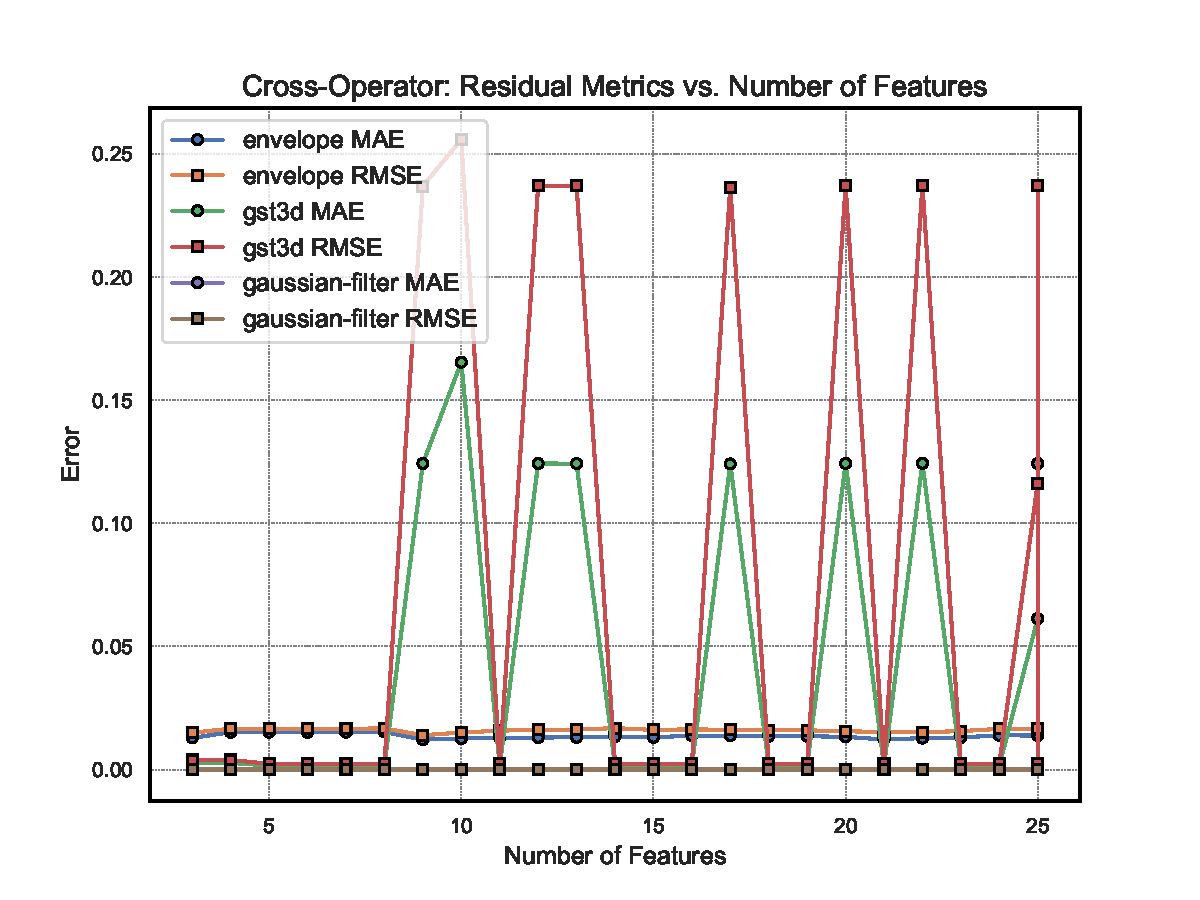
\includegraphics[width=\textwidth]{assets/images/05/residual_metrics_by_number_of_features}
        \caption{Residual metrics vs. number of features}
    \end{subfigure}
    \hfill
    \begin{subfigure}[t]{0.49\textwidth}
        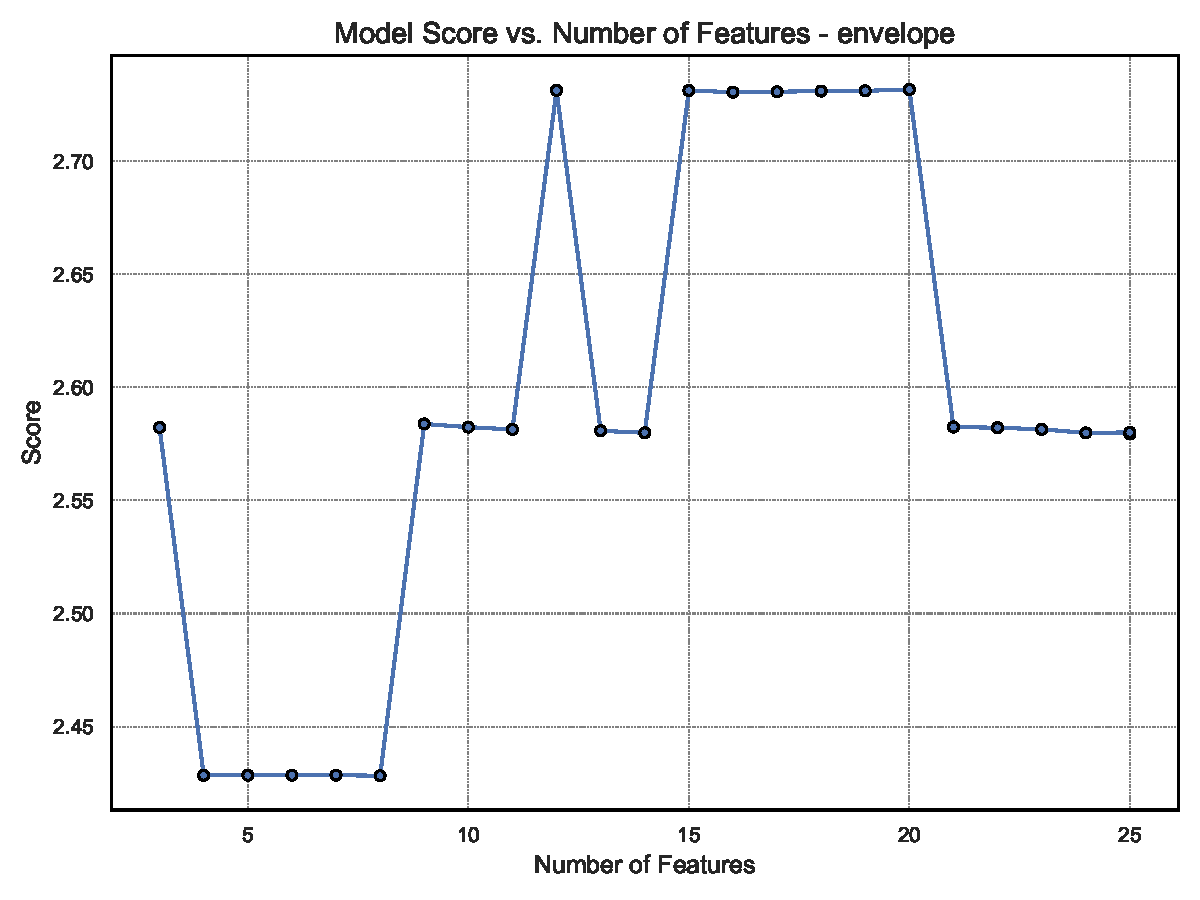
\includegraphics[width=\textwidth]{assets/images/05/score_by_number_of_features_envelope}
        \caption{Score for Envelope during reduction}
    \end{subfigure}
    \caption{Minimal degradation in residuals and scores with fewer predictors.}
    \label{fig:feature_selection_overview_part2}
\end{figure*}

\subsubsection{Operator-Specific Breakdown}
\label{subsec:operator-specific-breakdown}

Figures~\ref{fig:feature_impact_operator_subplots}--\ref{fig:residual_metrics_by_number_of_features_operator_subplots} confirm that Envelope and Gaussian Filter models maintain high accuracy using only volume.
\ac{GST3D} slightly benefits from one or two extra features, but volume remains the primary predictor.

\begin{figure*}[htbp]
    \centering
    \begin{subfigure}[t]{0.32\textwidth}
        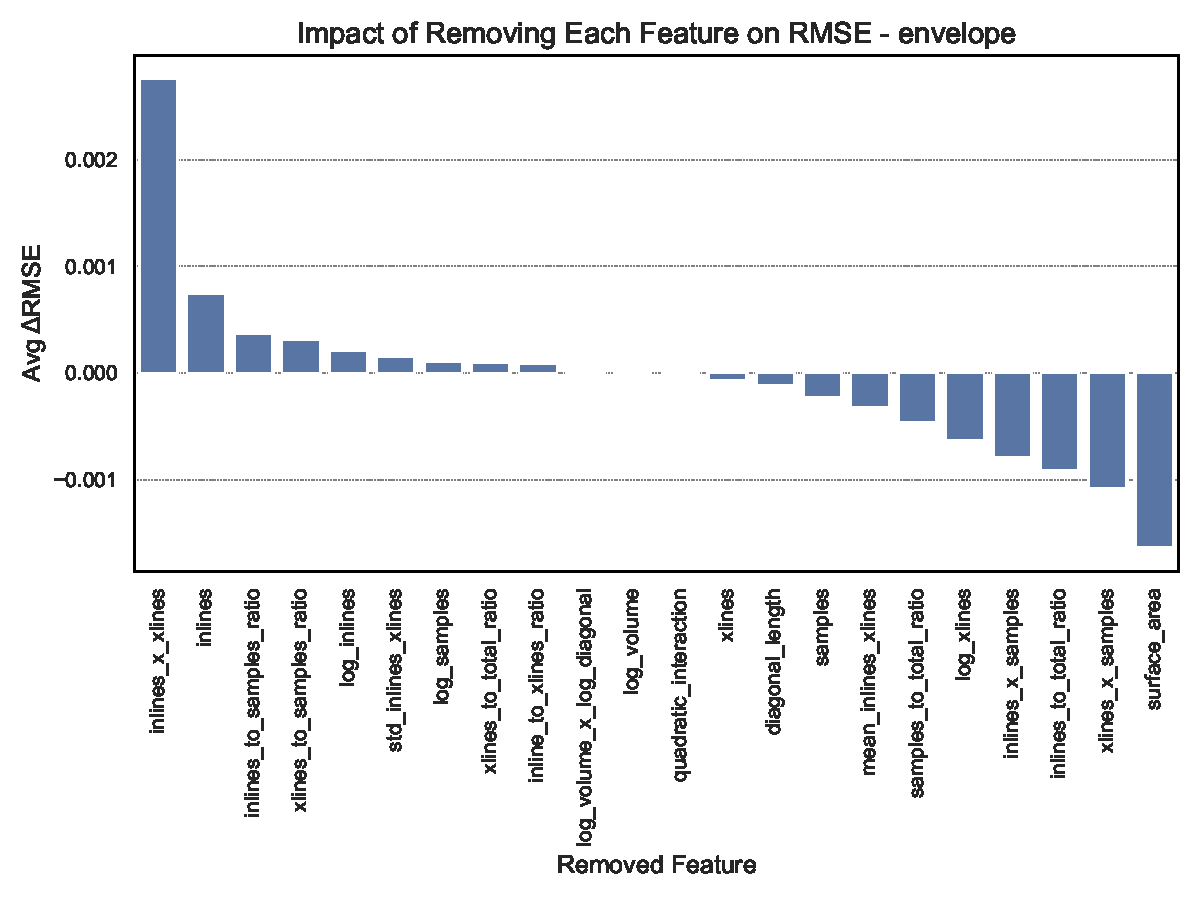
\includegraphics[width=\textwidth]{assets/images/05/feature_impact_envelope}
        \caption{Envelope}
    \end{subfigure}
    \hfill
    \begin{subfigure}[t]{0.32\textwidth}
        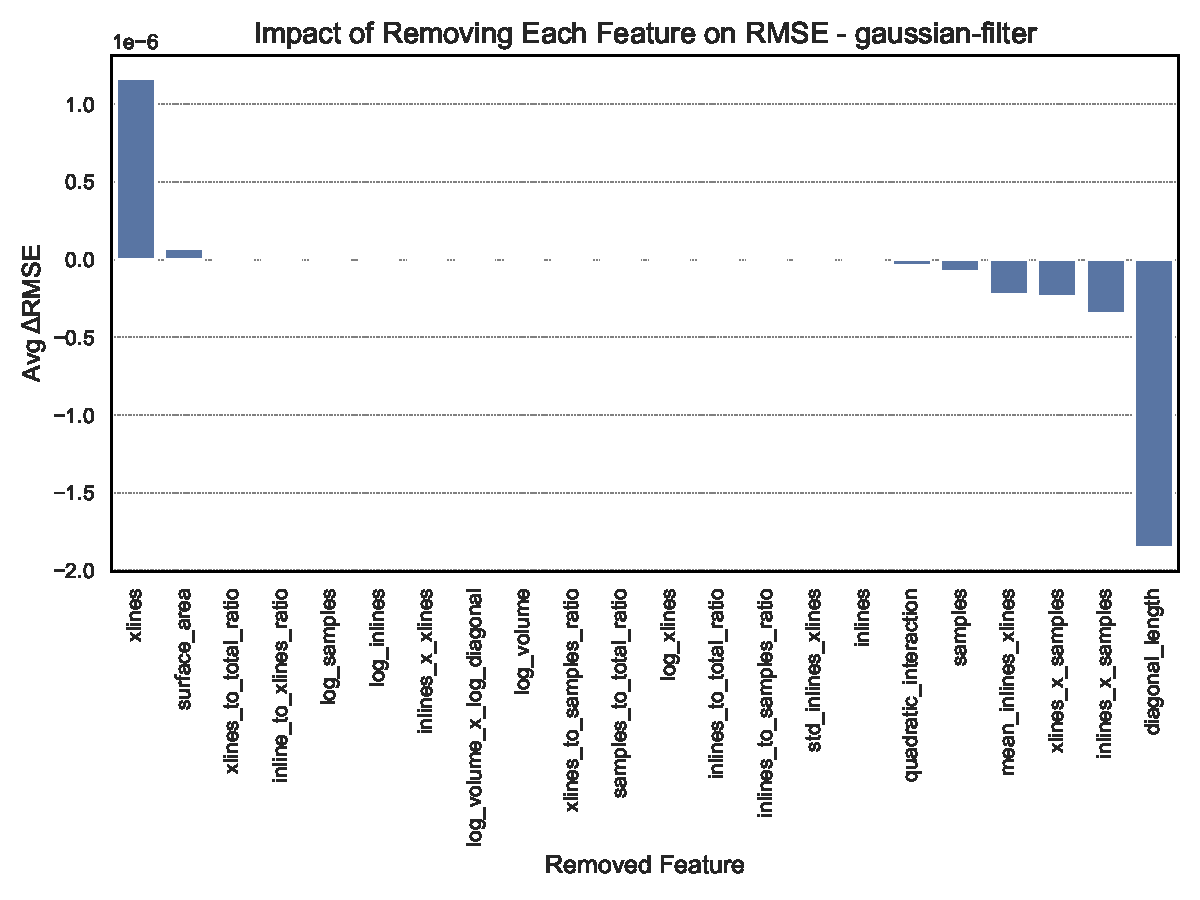
\includegraphics[width=\textwidth]{assets/images/05/feature_impact_gaussian-filter}
        \caption{Gaussian Filter}
    \end{subfigure}
    \hfill
    \begin{subfigure}[t]{0.32\textwidth}
        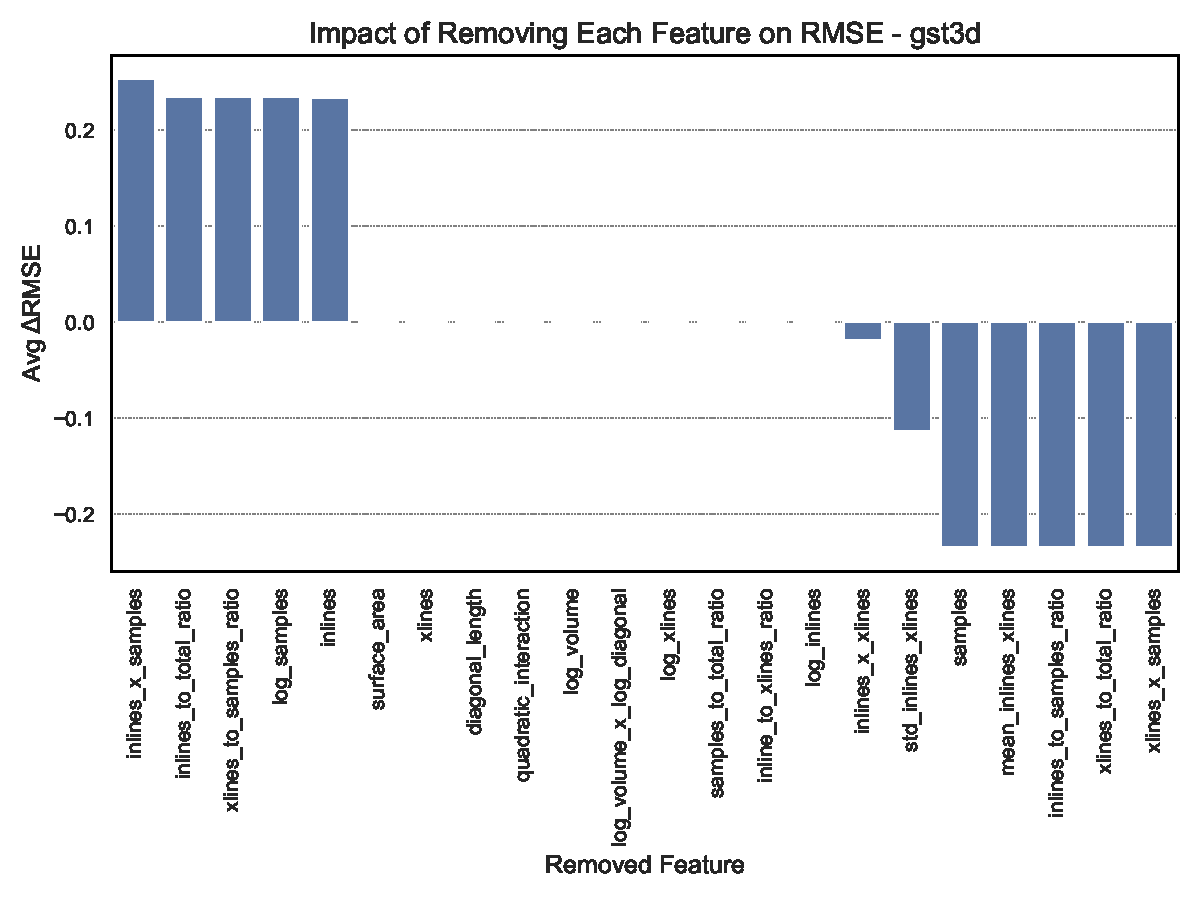
\includegraphics[width=\textwidth]{assets/images/05/feature_impact_gst3d}
        \caption{\ac{GST3D}}
    \end{subfigure}
    \caption{Performance drop when features are removed. Volume is most important across all operators.}
    \label{fig:feature_impact_operator_subplots}
\end{figure*}

\begin{figure*}[htbp]
    \centering
    \begin{subfigure}[t]{0.32\textwidth}
        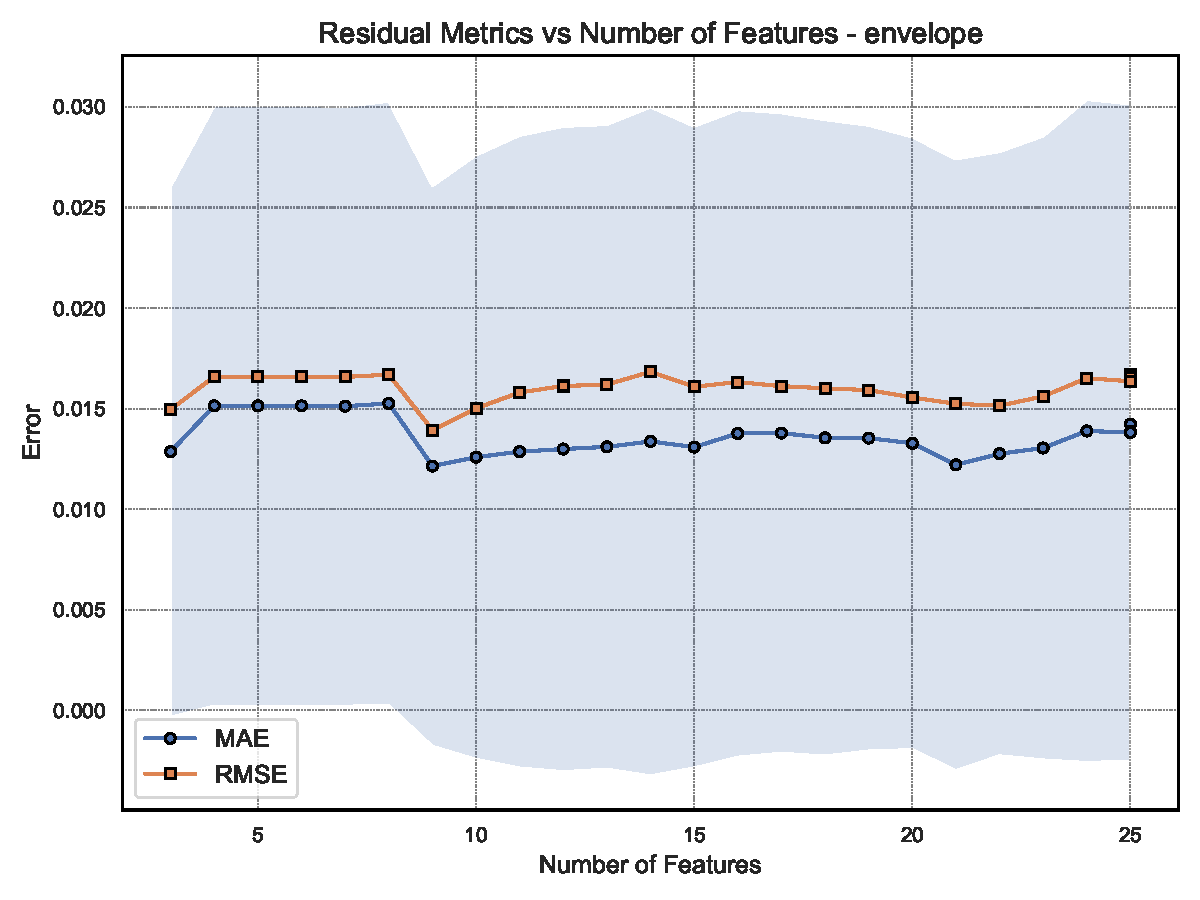
\includegraphics[width=\textwidth]{assets/images/05/residual_metrics_by_number_of_features_envelope}
        \caption{Envelope}
    \end{subfigure}
    \hfill
    \begin{subfigure}[t]{0.32\textwidth}
        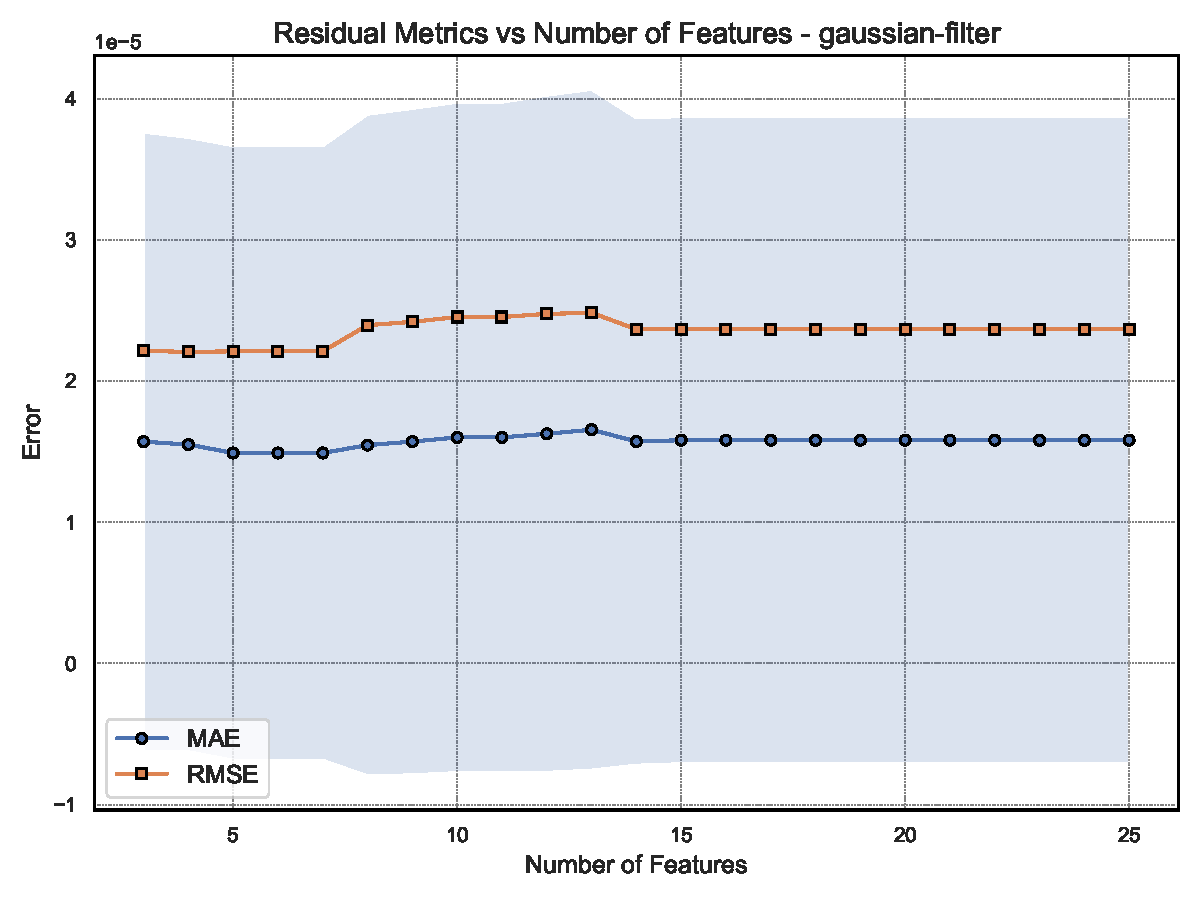
\includegraphics[width=\textwidth]{assets/images/05/residual_metrics_by_number_of_features_gaussian-filter}
        \caption{Gaussian Filter}
    \end{subfigure}
    \hfill
    \begin{subfigure}[t]{0.32\textwidth}
        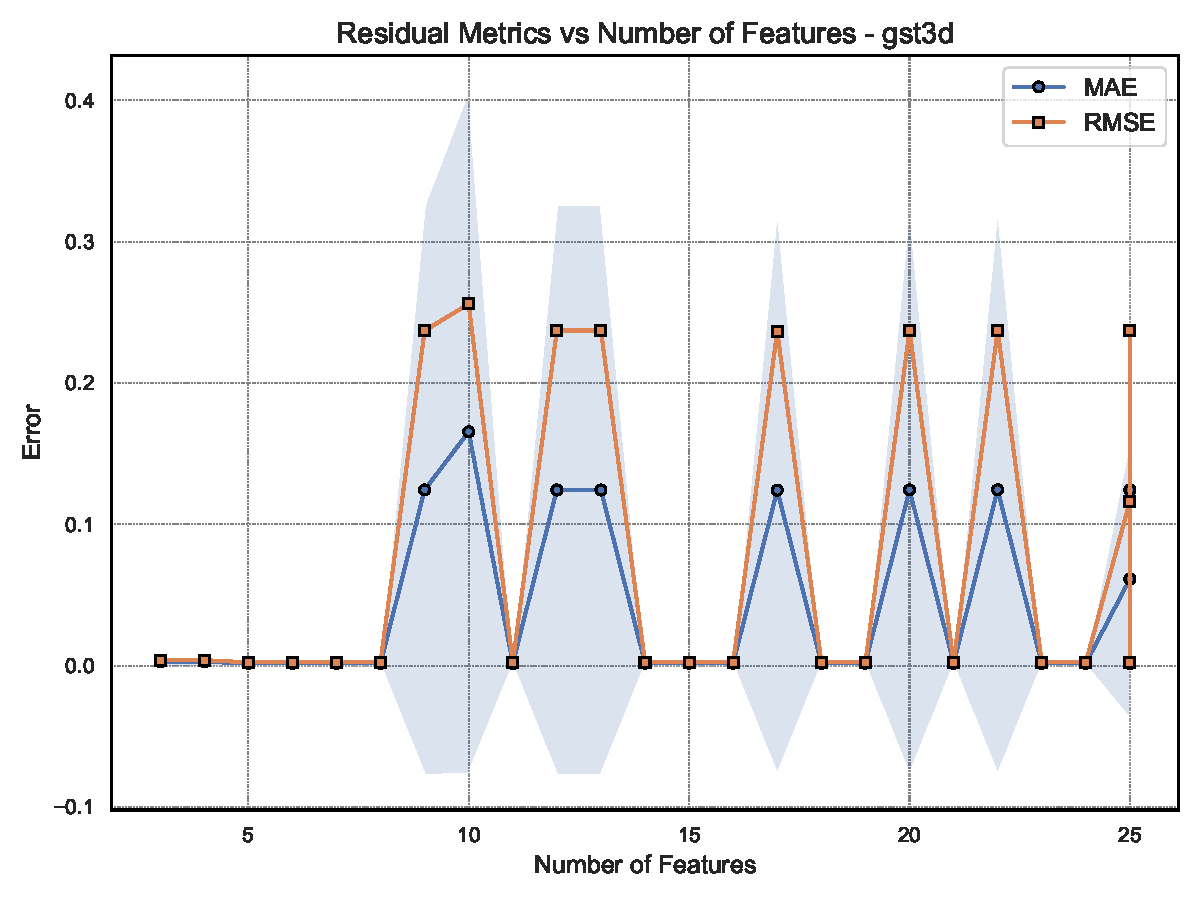
\includegraphics[width=\textwidth]{assets/images/05/residual_metrics_by_number_of_features_gst3d}
        \caption{\ac{GST3D}}
    \end{subfigure}
    \caption{Residual stability during feature removal. \ac{GST3D} sees slightly more fluctuation.}
    \label{fig:residual_metrics_by_number_of_features_operator_subplots}
\end{figure*}

\subsubsection{Summary of Findings}
\label{subsec:feature-selection-summary}

Volume alone provides high predictive power for all tested operators.
Other features offer marginal benefits, mostly for \ac{GST3D}.
Thus, memory-aware models can prioritize volume as the primary input.
